%=========================================================================
% (c) Michal Bidlo, Bohuslav Křena, 2008
\setcounter{secnumdepth}{4} % cislovani nadpisu do hloubky



\chapter{Úvod}
\label{chapter:1}

V současné době se technologie ve všech odvětvích stále posouvá a~není tomu jinak ani u~prohlížení fotek a~videí. V současné době i~takto nahrané informace pomocí digitálních zařízení je trend dále posouvat a~zvyšovat tak zážitek ze zaznamenané události. Díky tomuto trendu si už nevystačíme s ``klasickými''  přehrávači, popř. prohlížeči videí, nebo fotografií. Díky sférickým 360 stupňovým kamerám, je dnes možné zaznamenat video o~srovnatelné velikosti jako u dnes běžného telefonu, ale s~mnohem větším objemem informací, které se ale nedají srozumitelně přehrát v~klasických přehrávačích. Ruku v ruce se sdílením takových dát, je velice výhodné takový prohlížeč nabídnout jako webovou verzi, aby i~jiní uživatelé mohli svá takto natočená videa přehrávat popř. sdílet. Důkazem toho je rozmach multimediálního obsahu na internetu, kdy samotný jazyk HTML pro prezentaci webových stránek dříve nenabízel přímou podporu videí, což se změnilo příchodem nové verze HTML5. Některé portály jako např. Youtube již dnes začíná nasazovat do svého prohlížení videí jeho rozšířené sférické verze, což tedy potvrzuje tento trend. Tato práce má za cíl takové prohlížení posunout ještě dál.


Následující práce se věnuje implementaci webového prohlížeče panoramatických snímku a videí v různých módech, ve kterých je video interpretováno. Cílem je tedy navrhnout a zrealizovat řešení, aby uživatel po natočení videa dále nepotřeboval k přehrání např. sférického videa v režimu rybího oka specifický program, který by video musel nejprve překonvertovat. To stejné se týká i~panoramatických snímku a~videí v equirectangulárním zobrazení.  


Další inovací v prohlížení videí je přidání některých dat, které v běžném prohlížení nejsou k dispozici. Např. informace o světových stranách ve vztahu k obrázku, či videu popřípadě údaje o velikosti zorného pole v daném kontextu prohlížení až po dodatečná metadata v~panoramatických obrázcích, které jsou vhodné např. k~tomu, aby autor obrázku mohl popsat jeho zajímavé částí popřípadě blíže popsat zachycenou scénu.
\newline

Samotná práce je členěna do šesti částí. V kapitole \nameref{chapter:2} se budu věnovat nastínění všech použitých technologií nutných pro pochopení problematiky, se kterými se bude pracovat v následujících kapitolách. O návrhu řešení pojednává kapitola \nameref{chapter:3}, na kterou navazuje implementační část \nameref{chapter:4}. Otestování správného návrhu a implementace se zabývá kapitola s názvem \nameref{chapter:5}. V poslední části práce \nameref{chapter:6} jsou prezentovány dosažené výsledky a možnosti dalšího rozšíření.


%=========================================================================


\chapter{Webové technologie prohlížeče}
\label{chapter:2}
Následující kapitola pojednává o technologiích, které samotný prohlížeč používá a jsou tedy nezbytné v následujících kapitolách, zejména v části \nameref{chapter:4}, kde se s nimi přímo pracuje.


\section{HTML5}

Jazyk HTML (HyperText Markup Language) je značkovací jazyk určený pro popis webových stránek. Vychází z univerzálního značkovacího jazyka SGML (Standard Generalized Markup Language). V současné době aktuální verzi  jazyka HTML je jeho již pátá verze -  HTML5. Nová verze HTML přináší zásadní vylepšení, nové funkce a možnosti, které jsou nezbytné pro návrh a implementaci webového prohlížeče. 

Pro návrh samotného programu je nezbytná podpora multimédií – tedy audio a video, v neposlední řádě také plátno canvas sloužící pro práci s grafikou.



\subsection{Video}
Dříve nebylo možné do webových stránek vložit video tak jako dnes. K tomuto účelu bylo využíváno různých zásuvných modulů třetích stran a do webových stránek se video vkládalo např. jako objekt. Nejvíce rozšířeným přehrávačem videí a tedy jakási náhrada za podporu videí, kterou tehdy HTML nemělo, se v širším spektru stal Adobe Flash, který funkci přehrávače plní v menší míře až doposud, avšak je již zastíněn efektivnějším řešením, a to právě HTML5.

Nový prvek v HTML5 vytvořený k tomuto účelu je \texttt{<video>}. Byl navržen tak, aby mohl být použit bez detekčních skriptů na stránce. V elementu videa je možné nastavit více souborů s videem a dle podpory si daný prohlížeč vybere jim podporované video. V případě, že by prohlížeč prvek videa nepodporoval, bude jej ignorovat. Nastavení více zdrojů videa s odlišnými kodeky lze pomocí elementu \texttt{<source>} uvnitř páru elementů \texttt{<video>...</video>}. Jakmile prohlížeč narazí na \texttt{<video>}, podívá se, zdali je přítomen atribut \texttt{src}, v opačném případě začne procházet jeden element \texttt{<source>} po druhém a bude hledat právě takový, který umí přehrát.

Aby bylo možné ovládat video dynamicky pomocí kláves nebo myší, bude nutné využít DOM (Document Object Model). Jedná se o stromovou strukturu dokumentu, kterou si prohlížeč sestavuje po načtení webové stránky. Všechny elementy webové stránky jsou interpretovány v DOM jako objekt Některé značky se v DOM vytvoří, aniž by byly ve zdrojovém kódu zapsány. Obecně platí, že pomocí objektového modelu je díky javascriptu možné tuto stromovou strukturu dále upravovat a rozšiřovat. 



\subsubsection{Stavy načítání a přehrávání videa}
Další velice důležitou částí je načítáni videa a jeho ověření, zdali  je již video připraveno k přehrání. K ověření dostupnosti videa lze použít jeden ze síťových stavů elementu pomocí stavového atributu \texttt{networkState}, popřípadě přímo zjišťovat připravenost videa pomocí atributu \texttt{readyState} \cite{html5}, vracející jeden z následujících stavů, podle kterých se můžeme dále při přehrávání řídit a přizpůsobit tomu běh programu. Jednotlivé konstanty nabývají hodnot od \texttt{0} do \texttt{4} a dle hodnot rozlišujeme:


\begin{itemize}
	\item \texttt{HAVE\_NOTHING } (ekvivalentní hodnotě 0) \newline
	 - nastane v situaci, kdy zdrojové video není dostupné, nebo žádná data pro aktuální přehrávanou pozici \newline - koresponduje také s návratovou hodnotou síťové metody \texttt{networkState()}, když její návratová hodnota je rovna 0, což odpovídá konstantě \texttt{NETWORK\_EMPTY}
	\item \texttt{HAVE\_METADATA} \newline
		-  základní data o zdroji se podařilo získat a zdroj je tedy považován jako dostupný. Zatím ale ještě není dostatek dat, aby bylo možné začít s přehráváním. V tomto stavu jsou k dispozici jen data popisující přehrávány subjekt, jako délka, šířka, dekódovaní apod. Dochází k vyvolání události \texttt{loadedmetadata}
	\item \texttt{HAVE\_CURRENT\_DATA }\newline
		- data pro bezprostřední začátek přehrávání jsou připravena, ale video ještě není načteno dál za tuto pozici. Přehrávání může dostat do stavu \texttt{HAVE\_METADATA}, nebo následující data videa již nejsou k dispozici.
	\item \texttt{HAVE\_FUTURE\_DATA}\newline
		- data pro přehrávání jsou připravena pro současnou i nadcházející pozici. V případě, že by bylo video dosáhlo takového stavu poprvé, bude vyvolána událost \texttt{canplay}.
	\item \texttt{HAVE\_ENOUGH\_DATA}\newline
		- data připravena pro aktuální a nadcházející pozice pro plynulé přehrání. Dochází k vyvolání události \texttt{canplaythrough}
\end{itemize}

Mimo stavy načtení videa jsou tu i události indikující, co přesně se právě děje s videem po jeho načtení. Tyto stavy se hodí k dotazování elementu \texttt{<video>} pomocí DOMu např. pro tvorbu vlastního specifického ovládání videa, nebo pro zahrnutí interakce s myší.



\begin{itemize}
	\item \texttt{playing} - video se aktuálně přehrává, atribut \texttt{paused} je nastaven na \texttt{false}	
	\item \texttt{waiting} - přehrávání videa je pozastaveno, protože následující data videa nejsou k dispozici, webový prohlížeč ale očekává, že v vzápětí dostane
	\item \texttt{ended} - přehrávání videa doběhlo nakonec
	\item \texttt{canplaythrough} - tato událost říká, že je možné video přehrát až do konce bez nutnosti video zastavit k dalšímu načítání. Tohoto stavu může dosáhnout jen v případě, že stavový atribut \texttt{readyState} je roven \texttt{HAVE\_ENOUGH\_DATA}.
	
\end{itemize}

%=========================================================================
\newpage

\subsubsection{Atributy videa}
Důležité atributy pro manipulaci s videem a nastavením.



\begin{description}
	\item[src] - jedná se o atribut, do kterého se definuje zdrojové adresa videa jako URL, které se má zobrazit. Používá se zejména v situaci, kdy je k dispozici právě jedna verze videa.
	
	\item[autoplay] - jedná se atribut typu \texttt{bool}. V případě, že je \texttt{true}, spustí se přehrávání média automaticky jakmile je vše připraveno. Uvedení názvu atributu do elementu samotného je již dostačující informace o tom, co se bude dít s videem. Tedy bude tato hodnota typu \texttt{bool} považována jako \texttt{true}, jinak \texttt{false}.	
	
	\item[poster]  - Slouží k vystihnutí obsahu daného videa. Ještě než začne samotné přehrávání, je možné jako první snímek videa zvolit obrázek zadaný cestou. V~případe, že tento atribut nebude vyplněn, HTML automaticky zvolí jeden z prvních neprázdných rámců.
	
	\item[loop]  - jedná se atribut typu \texttt{bool}, který začne po dosažení konce videa s přehráváním videa opět od začátku. Tato operace se provádí v nekonečné smyčce.

	\item[width] - šířka přehrávače v pixelech.
	
	\item[height] - výška přehrávače v pixelech.

	\item[paused] - atribut videa typu \texttt{bool}. Indikuje, zdali se video přehrává či nikoliv.

	\item[controls] - jedná se opět o atribut typu \texttt{bool}, který říká, aby prohlížeč použil vlastní ovládací prvky pro video. Ovládací prvky se dají také vytvořit a přizpůsobit velice snadno díky DOMu.
 	
 	\item[preload]  - tímto říkáme, jakou část videa by měl webový prohlížeč načíst ihned po načtení stránky. Tento atribut nabývá jednou ze tří hodnot:
	 	\begin{itemize}
	 		\item \texttt{none} - nebude načítat nic, výhodné v případě, kdy je potřeba minimalizovat vytížení pásma	 		
	 		\item \texttt{metadata} - načte pouze metadata daného videa - základní údaje o jeho délce apod.
	 		\item \texttt{auto} - sám zvolí, co přesně udělá 
	 	\end{itemize}
\end{description}

%=========================================================================
\newpage

\subsubsection{Metody videa}
Jelikož pomocí DOM je možné upravovat vlastnosti elementu \texttt{<video>}, tak jsou tedy nutné metody k ovlivnění jeho atributů, aby bylo možné s přehráváním videa manipulovat.

\begin{description}
	\item[\texttt{play()}] - metoda sloužící k nastavení atributu \texttt{paused} na \texttt{false}, pokud video již skončilo, začne je přehrávat od začátku.
	\item[\texttt{pause()}] - metoda sloužící k nastavení atributu \texttt{paused} na \texttt{true}, tím dojde k pozastavení videa
	\item[\texttt{canplaytype()}] - metoda sloužící k ověření, zdali webový prohlížeč dokáže video daného typu přehrát. Metoda vrací jednu z následujících hodnot:
	 	\begin{itemize}		
			\item \texttt{""} - pokud by metoda vrátila prázdný řetězec, video prohlížeč nedokáže přehrát.
			\item \texttt{maybe} - prohlížeč si není zcela jist, zdali dokáže formát přehrát.
			\item \texttt{probably} - daný formát videa dokáže prohlížeč přehrát s vysokou pravděpodobností.
		\end{itemize}
	\item[\texttt{load()}] - všechny data videa se načtou znovu, čímž dojde ke zrušení všech akcí a současných dat, které byly doposud staženy a načteny. Poté se vše zavolá a načte znovu následujícím způsobem:
	 	\begin{enumerate}
			\item Nejprve dojde k inicializaci, kdy \texttt{readyState} je nastaven na \texttt{HAVE\_NOTHING} a  nastaví i příslušný síťový atribut \texttt{networkState} na \texttt{0}, \texttt{seeking} je nastaven na \texttt{false}, \texttt{paused} je nastaven na \texttt{true}, vše ostatní je prázdné, nebo nula	
			
			\item vybere se zdroj z atributu \texttt{src} nebo \texttt{<source>}, dále je vyvolána událost \texttt{loadstart} a dochází ke stažení metadat videa
			
			\item jakmile jsou metadata stažena, nastaví se zakladní vlastnosti videa - šířka, výška, délka a \texttt{readyState} je nastaven na \texttt{HAVE\_METADATA} a spolu s tím je vyvolána událost \texttt{loadedmetadata}
			
			\item Jakmile je \texttt{readyState} větší nebo roven \texttt{HAVE\_FUTURE\_DATA} je vyvolána událost \texttt{canplay} a \texttt{loadeddata}
			
			\item dojde ke spuštění přehrávání. Je vyvolána událost \texttt{play} a \texttt{playing}, atribut \texttt{paused} nastaven na \texttt{false}
		\end{enumerate}
\end{description}


%=========================================================================
\newpage

\subsection{Plátno}

Jak již bylo avizováno výše, plátno, neboli element \texttt{<canvas>} slouží v HTML5 pro vykreslení grafů, herní grafiky, obrazů bitmap apod. Díky elementu \texttt{<canvas>} lze vykreslovat i náročnější grafické objekty za pomocí WebGl. V HTML5 slouží tedy především k vykreslení 2D prvků pomocí Javascriptu. Plátno je párový  element, přesto se mezi párové tágy zdánlivě nic nevykresluje, celý obsah je skryt. Takový obsah se nazývá tzv. \textit{fallback content} a je zobrazen v případě chyby, nebo prohlížečům, které tento element HTML5 nepodporují.

Plátno je bezpochyby nejdůležítější částí pro realizaci celé práce. Bude pro vyobrazení používat především \texttt{<video>}, z kterého bude číst data a využije tedy element video jak zdroj. Díky DOM pak dokážeme s objektem snadno manipulovat. Díky elementu \texttt{<canvas>} jsme tedy schopni získat kontext Javascriptového API - WebGl a díky němu schopni pracovat na úrovni grafické karty.

\subsubsection{Atributy plátna}
Canvas má pouze dva atributy a těmi jsou \texttt{width} a \texttt{height} pro nastaveni šířky a výšky plátna. Je možné nastavit výšku a šířku pomocí kaskádových stylů, avšak tato možnost není doporučována, protože by mohlo dojít k nežádoucí deformaci obsahu. Při změně velikosti bitmapy pomocí atributů dojde pouze ke změně velikosti dané bitmapy, změna kaskádovými styly ale změní velikost obsahu celé bitmapy a tím tedy dojde ke zkreslení.

\subsubsection{Použití a práce s plátnem}
Použit plátno lze pomocí rozhraní \texttt{HTMLCanvasElement}, které slouží pro přístup k jeho vlastnostem a metodám. Přístup k objektu \texttt{HTMLCanvasElement} lze pomoci standardní javascriptové metody \texttt{getElementById()} v případě, že je v tágu \texttt{<canvas>} nastaven atribut \texttt{id}, nebo lze objekt získat pomocí metody \texttt{querySelector("canvas")}.

Po získání objektu plátna lze dále s elementem manipulovat pomocí dvou metod (počet volání dané metody vrátí pokaždé ten stejný objekt):
	 	\begin{itemize}		
			\item \texttt{ toDataURL([type[,quality]])} \cite{html5}\newline
			 - vrací URL adresu aktuálního obrázku v elementu \texttt{<canvas>}. Metoda může a nemusí mít nějaké argumenty. První argument, v případě že je zadán, rozhoduje jaký bude navrácen výsledný typ obrázku. Pokud nezadáme žádný argument, tak jako výchozí formát obrázku bude automaticky zvolen \textit{image/png}. Výsledná adresa URL bude vrácena jako řetězec.
			\item \texttt{getContext(contextId[, ... ])}\newline
			 - metoda vrací referenci na daný objekt aplikačního rozhraní, díky kterému bude možné kreslit na plátno. Pokud by kontext pro daný argument nebyl podporován prohlížečem, návratová hodnota bude \texttt{null}. Typ aplikačního rozhraní je vybrán na základě argumentu metody:
			 \begin{itemize}
			 	\item  \texttt{\textbf{"2d"}} - vrací objektové rozhraní \texttt{CanvasRenderingContext2D}, kterí slouží pro kreslení grafických primitiv.
			 	\item \texttt{\textbf{"webgl"}} - pokud tuto funkci prohlížeč podporuje, bude navrácen objekt \newline \texttt{WebGLRenderingContext}. 
			 \end{itemize}
		 
 
		\end{itemize}

%=========================================================================
\newpage


\subsection{Vektory}
SVG (Scalable Vector Graphics) - škálovatelná vektorová grafika je již zažitý standard. Doposud ale nebylo možné kód \texttt{svg} vkládat přímo do HTML. Změna přišla až s HTML5. SVG vychází z jazyka XML (e\textbf{X}tensible \textbf{M}arkup \textbf{L}anguage)\footnote{obecný značkovací jazyk pro serializaci dat.}. Mezi jeho nesporné výhody patří velikost, přenositelnost a nezávislost na rozlišení aj. Do HTML se vkládá pomocí elementu \texttt{<svg>}, který má zpravidla dále zanořené elementy, které reflektují jeho obsah. Mezi takové vnořené elementy patří take tág \texttt{<path>}.


\subsubsection{Element path}
Generický element \texttt{<path>} slouží ve vektorové grafice k vytvoření křivky, která může být dále vyplněna barvou, nebo může sloužit k vytvoření ořezové cesty apod. Dále může mít nastaveny atributy specifikující vykreslování obrysů, nastavení stylů a tříd, nebo nastavení kalkulace délky cest. Mezi takové atributy patří:

\begin{description}
	\item[d]  - tento atribut nese informace o cestě, resp. data k vyrekslení obrysu, který poté můžeme vyplnit konkrétní barvou, popř. jej využít k dalším podobným účelům víz výše. Data atributu se skládají z následujících částí:
	\begin{itemize}
		\item \texttt{\textbf{M}}/\texttt{\textbf{m}} (\textit{moveto}) její syntaxe: \texttt{\textbf{M x y}} nebo \texttt{\textbf{m x y}} - realizuje posun na danou dvojice souřadnic \texttt{(x, y)} bez kreslení. Velké písmeno \texttt{M} značí, že souřadnice budou absolutní. Malé písmeno \texttt{m} indikuje, že budou souřadnice relativní\footnote{Velikost písmen má stejný význam u všech příkazů.}. Tuto vlastnost je velice výhodné používat pro všechny cesty, jinak by vždy následující čára začínala na konci té předchozí.\\
		
		\item \texttt{\textbf{Z}}/\texttt{\textbf{z}} (\textit{closepath}) - tento příkaz je bez parametrů a slouží k uzavření cest, tedy spojení posledního bodu s prvním bodem vykreslovaných cest.\\
		
		\item \texttt{\textbf{L}}/\texttt{\textbf{l}} (\textit{lineto}) - tento příkaz již kreslí čáru, jeho syntaxe je  stejná jako u příkazu \textit{moveto} tj \texttt{L/l x,y}\\
		
		\item \texttt{\textbf{H}}/\texttt{\textbf{h}} (\textit{horizontal lineto}) - kreslí horizontální čáru z bodu (cp\textbf{x}, cp\textbf{y}) to (\textbf{x}, cp\textbf{y}), argument příkazu je pouze souřadnice \texttt{x}\\
		
		\item \texttt{\textbf{V}}/\texttt{\textbf{v}} (\textit{vertical lineto}) - kreslí vertikální čáru z bodu (cp\textbf{x}, cp\textbf{y}) to (cp\textbf{x}, \textbf{y}), argument příkazu je pouze souřadnice \texttt{y}\\
		
		\item \texttt{\textbf{A}}/\texttt{\textbf{a}} (\textit{elliptical arc}) - parametry:  \textit{{\small (rx ry x-axis-rotation large-arc-flag sweep-flag x y)}} \\ kde \texttt{rx} značí první poloměr elipsy, \texttt{ry} druhý poloměr, \texttt{x-axis-rotation} rotace kolem osy x, příznak \texttt{large-arc-flag} značí, zdali bude oblouk krátký (hodnota \texttt{0}) popř. dlouhý (hodnota \texttt{1}), dále argument \texttt{sweep-flag} příznak značící oblouk proti směru/po směru (\texttt{0}/\texttt{1}), \texttt{x} a \texttt{y} souřadnice koncového bodu
	\end{itemize}


	\item[fill]  - vyplní křivku zadanou argumentem \texttt{d} libovolnou barvou
\end{description}




%=========================================================================
\newpage

\section{GLSL}
\textbf{GLSL} (Open\textbf{GL} \textbf{S}hading \textbf{L}anguage) - jedná se o jazyk pro psaní shaderů \footnote{Jedná se o programy řídící vykreslování na grafické kartě.}. Jazyk vychází z jazyka C a také proto je mu svojí syntaxí velice podobný. Základní konstrukce každého programu je v zásadě úplně stejná jako v jazyku C, každý program musí obsahovat hlavní funkcí \texttt{main()} bez jakýkoliv parametrů a návratových hodnot. V hlavní funkci programu jsou vyhrazeny proměnné se speciálním významem, jako např. \texttt{gl\_Position}, kterou nastavujeme  pozici vrcholu ve vertex shaderu, nebo \texttt{gl\_FragColor} pro nastavení barvy ve fragment shaderu.

\subsection{Vertext shader}
Jedná se o program v jazyce GLSL, který je pro prováděn pro každý vstupní vrchol zadané geometrie. 

Každá souřadnice vrcholu je dále přepočítána do tzv. \textit{clipspace}, což je souřadný systém pro vykreslování do plátna. V případě, že by některé souřadnice byly mimo hranice souřadného systému, budou oříznuty a vykreslovat se nebudou. Hranice \textit{clipspace} jsou definovány pro každou ze souřadnic \texttt{x},\texttt{y}, \texttt{z} intervalem \texttt{<-1,1>}. Vertex shader může sám ovlivnit souřadnice vrcholů, textur popř. normálových vektorů a barev. Při zpracování vrcholů není známa topologie zpracovávaného objektu, protože nejsou dostupné informace o sousedících vrcholech. 

Poslední operací vertex shaderu před samotným vykreslením je převod do NDC\footnote{Normalized Device Coordinates.} \cite{opengl}. Rozdílné operační systémy mají rozdílné způsoby reprezentace grafických objektů. Zabránit těmto rozdílným  intepretacím v praxi znamená, že se souřadnice \texttt{x}, \texttt{y} a \texttt{z} vydělí homogenní souřadnici.

\subsection{Fragment shader}
Je program - označovaný taktéž jako \textit{pixel shader}, který je volán pro každý pixel vykreslované scény. Jeho úkolem je výpočet barvy každého pixelu a díky tomu lze s takto získanou barvou  dále pracovat. Barva je získána jako čtyřsložkový vektor, první tří složky tvoří paletu RGB, poslední čtvrtá složka tvoří $\alpha$ kanál \footnote{Složka pixelu udávající jeho průhlednost.}. V případě vykreslování složitějších objektů umožňuje GLSL automaticky body geometrie interpolovat, tedy automaticky získat pixel dané geometrie, aniž by musel být každý samostatně definován. Ukázka interpolace je demonstrována na obrázku \ref{img:1}.

%=========================================================================
\newpage


\subsection{Typy proměnných}
Předávání hodnot v globálních proměnných může probíhat za pomocí třech datových typu, těmi jsou:
\begin{description}
	\item[\texttt{uniform}]  
	- uchovává hodnoty, které jsou konstantní po celou dobu běhu programu. Využívá se např. pro data transformačních matic apod.	
	\item[\texttt{attribute}] 
	- 	jedná se o vstupní data vertex shaderu, která mění svoje hodnoty pro každý vrchol. 
	\item[\texttt{varying}] 
	- tento datový typ slouží k předávání hodnot z vertex shaderu do fragment shaderu. Pomocí něj se provádí výše avizovaná interpolace, viz. obr. \ref{img:1} 

\end{description}


 
\begin{figure}[h]
	\label{img:1}
	\centering
	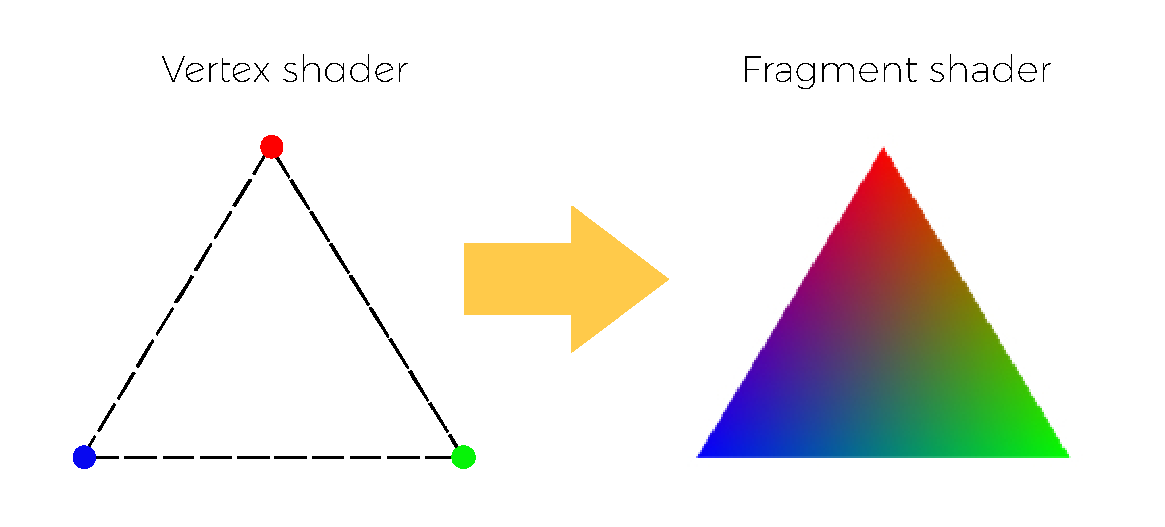
\includegraphics[scale=1.0,angle=0,width=1.0\linewidth]{obrazky-figures/interpolace}
	% 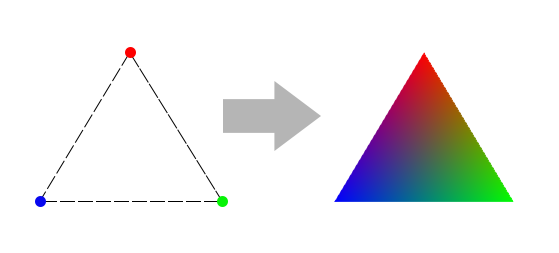
\includegraphics[scale=1.0,height=2.5in,angle=0]{obrazky-figures/interpolace.png}
	\caption{Ukázka interpolace hodnot mezi vertex a fragment shaderem.}
	\label{fig:inter}
\end{figure}
 



%=========================================================================
\newpage

\section{WebGL}
WebGL (\textbf{Web} \textbf{G}raphics \textbf{L}ibrary) je javascriptové aplikační rozhraní, které slouží pro nativní vykreslování 2D a 3D interaktivní grafiky přímo z webového prohlížeče \cite{mozilla}. K samotnému běhu WebGL není potřeba žádných dodatečných knihoven, nebo zásuvných modulů, protože je v tomto ohledu využívána přímo grafická karta. Program WebGL se v zásadě skládá z více jazyků, přičemž každý mů svůj vlastní účel a je nutné je používat dohromady. Jedním z nich je javascript, druhý je jazyk GLSL. V jazyce GLSL jsou napsány dva programy - vertex shader a fragment shader. Oba programy kompiluje ovladač grafické karty do kódu, který je poté vykonáván přímo na grafické kartě. Vertex shader i fragment shader mohou být předávány jako řetězce, takže manipulace s nimi je díky tomu značně zjednodušena. Velkou výhodou WebGL je integrace s DOM tudíž od automatické správy pamětí přes zpracování událostí až po jednoduché načítání bitmapy přímo v prostředí prohlížeče apod.. Zpracování všech dat i samotný běh programu je z hlediska implementace velice podobný konečnému automatu. 

K samotnému vykreslení je použit již výše zmíněný element HTML5 \texttt{<canvas>}, ze kterého se získá WebGL kontext.

V současné době je oficiálně vydána verze WebGL 1.0, která je založeno na OpenGL ES 2.0. Doposud se jedná o jedinou stabilní verzi. OpenGL ES\footnote{OpenGL for Embedded Systems.} je zjednodušená verze OpenGL, která eliminuje většinu vykreslovacích pipeline. Tato verze je především určena pro menší vestavěné systémy. Dalším rozšířením WebGL bude verze 2.0, která se stále nachází ve vývoji. Bude založena na OpenGL ES 3.0 přinášející velká vylepšení v zobrazování 3D grafiky - zejména textur, akceleraci vizuálních efektů, novou verzí jazyka GLSL s plnou podporu desetinných a celočíselných operací apod.



\subsection{Vykreslování primitiv}
K vykreslení nějakého grafického prvku jsou potřeba v zásadě jen dvě věci - vrcholy přepočítané do tzv. \textit{clipspace} a jemu přiřazené odpovídající barvy. Jak pro vrcholy tak pro barvy slouží jiný GLSL shader. K vyobrazení objektu používá WebGL tří základní primitiva - vykreslení samotných bodů, čar nebo trojúhelníku. Vše funguje tak, že zadaný bod, kterému budeme chtít přiřadit barvu, se načte do odpovídající speciální globální proměnné ve vertex shaderu, tam se daná hodnota přepočítá do intervalu \texttt{<-1,1>} pro všechny jeho osy a vzniklá hodnota se uloží na grafické kartě. Počet bodu záleží na primitivu, které vykreslujeme. Pokud se tedy jedná o bod, stačí pouze jeden bod ve vertex shaderu, pokud se jedna o čáru tak dvě popř. trojúhelník, tak trojice bodů. GPU\footnote{Graphic Processing Unit - grafický procesor} poté zjistí, které pixely korespondují s vykreslovaným primitivem a pro každý takový pixel zavolá fragment shader. 


\subsection{Vyrovnávací paměť}
Buffery resp. vyrovnávací paměti jsou rychle přístupné paměti na grafické kartě. V bufferech jsou  uloženy potřebné data k vykreslování grafických objektů jako např. body geometrie, normály, mapování textur apod. Data jsou poté snadno dále předávány GLSL shaderům, které s nimi pracují.


%=========================================================================
\newpage

\subsection{Projekce}
Některé frameworky\footnote{Rámcová softwarová struktura usnadňující řešení dané problematiky} založené na WebGL zaměňují projekci za kameru, ta bohužel jako taková ve WebGL neexistuje. Jedná se pouze o způsob vykreslení grafické informace, ke které jsou využívány právě projekční zobrazení. WebGL podporuje dva základní typy projekce - ortografickou a perspektivní. 

Ortografická projekce využívá skutečné velikosti objektu. Scéna je reprezentována jako pravoúhlý hranol.

Perspektivní projekce zkresluje velikost objektů způsobem, jak je tomu v reálném světě. Čím je objekt dál od pozorovatele, tím se bude jevit jako menší, protože jeho pozice je středem této projekce. Dalším příkladem bychom mohli uvést koleje, které se v dálce jeví, jakoby se sbíhaly v jednu jedinou apod.
  
Pokud bychom chtěl vykreslit nějaký 3D objekt, bude potřeba mít v bufferech informace o vrcholech, normálách, textuře apod. Tyto data bychom zároveň museli neustále aktualizovat a nahrávat zpět do paměti, aby bylo možné s daným 3D objektem jakkoli manipulovat, posouvat apod., aby nedocházelo k neustálému přepisování hodnot v paměti na GPU. Veškeré změny zrealizujeme transformačními maticemi, kterými se bude geometrie objektu v paměti násobit, aniž by data v paměti byla jakkoli změněna.

\subsection{Homogenní souřadnice}
Homogenní souřadnice je tvořena čtyřmi prvky - \texttt{x}, \texttt{y}, \texttt{z} a \texttt{w}. První tři složky tvoří souřadnice euklidovského prostoru, poslední prvek \texttt{w} je perspektivní složka a spolu se souřadnicemi \texttt{x}, \texttt{y}, \texttt{z} tvoří projekční prostor.\cite{WebGLbeg}

Perspektivním dělením - vydělením souřadnic \texttt{(x, y, z)} perspektivní složkou \texttt{w}, lze získat normalizované hodnoty bodu zpět do trojrozměrného souřadného systému. Platí zde ale, že perspektivní složka nesmí být nulová. 

Samotná perspektivní složka funguje v homogenních souřadnicích jako změna měřítka daného bodu geometrie.

Jednou z dalších vlastností homogenní souřadnice je ta, že umožňuje definovat body do nekonečna, resp. nekonečnou délku vektoru, což ve standardním trojrozměrném prostoru možné není. Tato situace nastává v případě, kdy je složka rovna nule.

\subsection{Model matrix}
Jedná se o matici, kterou držíme pro každý vykreslovaný objekt. Stará se o úpravu tvaru, natočení a posuvu objektu.

\subsection{View matrix}
Díky teto transformační matici realizujeme již avizovanou ``roli kamery'' , kdy simulujeme vzájemná vztah scény a pozorovatele.

\subsection{Perspective matrix}
Stará se o perspektivní zkreslení scény. Tato transformace rozhoduje o tom, jak velké zorné pole bude vykresleno a mapováno 
na obrazovku monitoru. 

%=========================================================================
\newpage

\subsection{Vytvoření a běh programu}
Po vytvoření kontextu \texttt{webgl} je již možné využívat funkce pro práci s WebGL. Funkce by se daly rozdělit na několik částí, nejprve ty, které pracují s shadery, dále ty které vytváří program, v neposlední řadě funkce pro prací s buffery a vykreslením dat. Všechny funkce WebGL pracují nad vytvořeným kontextem plátna\footnote{Vytvořený WebGL kontext budeme označovat jako \texttt{gl}}.

\begin{description}
	\item[\texttt{gl.createShader(type)}] - vytvoří objekt shaderu, vstupním argumenty \texttt{type} mohou být \\ \texttt{gl.VERTEX\_SHADER} nebo \texttt{gl.FRAGMENT\_SHADER}
	
	\item[\texttt{gl.shaderSource(shader, source)}] - asociuje objekt shaderu \texttt{shader} se zdrojovým kódem samotného shaderu \texttt{source} v textové formě
	
	\item[\texttt{gl.compileShader(shader)}] - kompiluje GLSL kód na binární data, vstupním parametrem je objekt shaderu \texttt{shader}
	
\end{description}

Následuje práce s programem. Funkce \texttt{gl.createProgram()} vytvoří objekt programu. Poté \texttt{gl.attachShader(program, shader)} - přiloží daný shader k programu.
Funkce \\ \texttt{gl.linkProgram(program)}, která slinkuje vše dohromady, \texttt{gl.useProgram(program)} - nastaví daný webgl program jako část současného vykreslovacího stavu.

\begin{description}
	
	\item[\texttt{gl.getAttribLocation(program, attribute)}] - vrací referenci na atribut v ve vertex shaderu
	
	\item[\texttt{gl.enableAttribute(attribute)}] - aktivuje atribut 
	
	\item[\texttt{gl.createBuffer()}] - vytvoří nový buffer objekt pro data
	
	\item[\texttt{gl.bindBuffer(target, buffer)}] - nastaví vytvořený buffer \texttt{buffer} jako aktivní, parametr \texttt{target} specifikuje data s jakými se bude pracovat
	
	\item[\texttt{gl.bufferData(target, srcData, usage)}] - parametr \texttt{target} má stejný význam jako u funkce \texttt{bindBuffer}, \texttt{srcData} určuje data, která se nahrají do bufferu, poslední parametr \texttt{usage} specifikuje způsob využiti uložených dat
	
	\item[\texttt{gl.vertexAttribPointer(attrib, size, type, normalized, stride, offset)}] -  \texttt{attrib} prováže atribut programu s aktivním bufferem, \texttt{size} určuje, z kolika prvků se skládají data v bufferu, \texttt{type} spcecifikuje datový typ dat v bufferu, \texttt{normalized} určuje zdali budou hodnoty normalizovány, parametr je typu \texttt{bool}, dále \texttt{stride} udávající zdali budeme nějaké hodnoty přeskakovat, \texttt{offset} odkud budeme data číst.
	
	
\end{description}

Samotné vykreslení uložených data v bufferech se realizuje funkcemi:


\begin{description}
	
	\item[\texttt{gl.drawArrays(mode, first, count)}] - vykresluje vstupní data. Parametr \texttt{mode} určuje, jaké grafické primitivum budem použito pro vykreslení, \texttt{first} určuje odkud se data zažnou upracovávat, \texttt{count} specifikuje počet vykreslovaných hodnot
	
	\item[\texttt{gl.drawElements(mode, count, type, offset)}] - stejně jako u \texttt{drawArrays()} určuje vykreslované grafické primitivum, to stejné se týká i parametru \texttt{count}, \texttt{type} definuje typ dat indexů a \texttt{offset} odkud začínáme zpracovávat indexy. HLavním rozdílem vůči funkci \texttt{drawArrays()} je ten, že \texttt{gl.drawElements(...)} nevykresluje body přímo, ale dostává jako vstupní data indexy na jednotlivé body, které vykresluje funkce \texttt{drawArrays()}
	
\end{description}

%=========================================================================
\newpage

\chapter{Návrh klíčových částí}
\label{chapter:3}
Kapitola nastiňuje, jakým způsobem jsou řešeny nejzásadnější problémy implementace prohlížeče. Snaží se navrhnout ty nejefektivnější způsoby řešení daných problémů a v případě, že tomu tak v konkrétním případě není, snaží se tyto  kroky návrhu jasně odůvodnit, proč jsou  daným způsobem takto řešeny.


\section{Geometrie}
Geometrie je potřebná k mapování textury, a to tak, aby daná textura reflektovala scénu co nejvěrněji. Kdybychom pro texturu nevytvářeli geometrii, na kterou se bude mapovat a jednoduše data namapovali do libovolné 2D roviny, dojde k významnému zkreslení pořizované scény.

K vyobrazení geometrie budeme využívat klasické pole, kde každý bod bude tvořen třemi rozměry v kartézské soustavě souřadnic, tedy formátu \texttt{[x1,y1,z1, x2,y2,z2, …]}, které utváří jednotlivé body v 3D prostoru. Body pak mezi sebou tvoří prostor, na který budou texturovací data  mapovaná. Ve WebGL umíme vykreslit jednotlivé body, čáry – tedy spojnice jednotlivých bodů, nebo trojúhelníky. V našem případě bude potřeba vykreslit texturu jako plochu, na kterou se bude vše mapovat. Pro ten to případ se ve WebGL používá vykreslení pomocí trojúhelníku, jako základní vykreslované primitivum plochy.

Geometrickým tělesem pro mapování bude zvolena koule, protože scéna resp. pořízená data, která budeme zpracovávat jsou zachycena ve sférickém modu a mapováním na kouli je dosažena nejvěrnější reprezentace scény.

Kouli so rozdělíme na poledníky a rovnoběžky. Poledníkem je v tomto případě myšlena spojnice severního a jižního pólu, kde úhel z počátku kartézské soustavy souřadnic mezi jednotlivými poledníky nabývá hodnot od 0 - 360\degree. Rovnoběžkou je myšlena kružnice  rovnoběžná se vzájemně sousedícími a svírající úhel s počátkem souřadnic od 0-180\degree. 

Je třeba tedy nejprve stanovit počet poledníků a rovnoběžek a z takových hodnot bude dále vypočítán úhel. Na základě úhlu budeme schopni přesně definovat bod v trojrozměrné rovině. Čím větší počet rovnoběžek a poledníků, tím bude geometrie věrněji aproximovat kouli - zvýší se hustota bodů v bufferech a tím bude i samotné vykreslení náročnější. Proto je ideální kompromis mezi jemností bodů a rychlosti načítání s téměř stejným výsledkem. Tato vlastnost by se nám hodila hlavně tedy v případech, kdy bychom měli vykreslit rozmanitý geometrický objekt se spoustou detailních sekvencí. V našem případě tento rozdíl tedy nepůjde okem rozeznat, takže skrze efektivitu je výhodné spíše snížit počet rovnoběžek a poledníků, čímž dosáhneme pozitivního efektu na samotnou rychlost programu.


\subsection{Sférický souřadný systém}

Každá rovnoběžka má po svém obvodu průsečíky s jednotlivými poledníky, tyto průsečíky jsou naše body geometrie, které budou nahrány do bufferů. Jelikož každá rovnoběžka nabývá úhlu od 0 do 180\degree  resp. $0-\pi$, tak tento úhel můžeme podělit počtem rovnoběžek a vynásobit aktuální rovnoběžkou, čímž získáme svíraný úhel s počátkem souřadnic. Na obrázku \ref{fig:geom} označujeme tento úhel jako $\theta$. Provedením této operaci pro všechny horizontální obvodové kružnice, vypočítáme všechny svírané úhly s počátkem souřadnic. 

Dále je nutné vypočítat svíraný úhel všech poledníků - vertikálních čar svírajících jej s počátkem souřadnic. Na obrázku \ref{fig:geom} je vyznačen jako $\varphi$. Jak jsem již nastínil výše, $\varphi$ nabývá hodnot od 0 do 360\degree resp. $0-2\pi$. Vytyčený úhel mezi jednotlivými čarami jsme schopni spočítat tak, že jej podělíme počtem vertikálních čar a vynásobíme aktuálním poledníkem. Takto získáme rovnoměrné rozložení bodů na celé rovnoběžce. Provedením  operace pro všechny rovnoběžky již bude geometrie koule z hlediska úhlů kompletní.

\begin{figure}[h]
	\label{img:2}
	\centering
	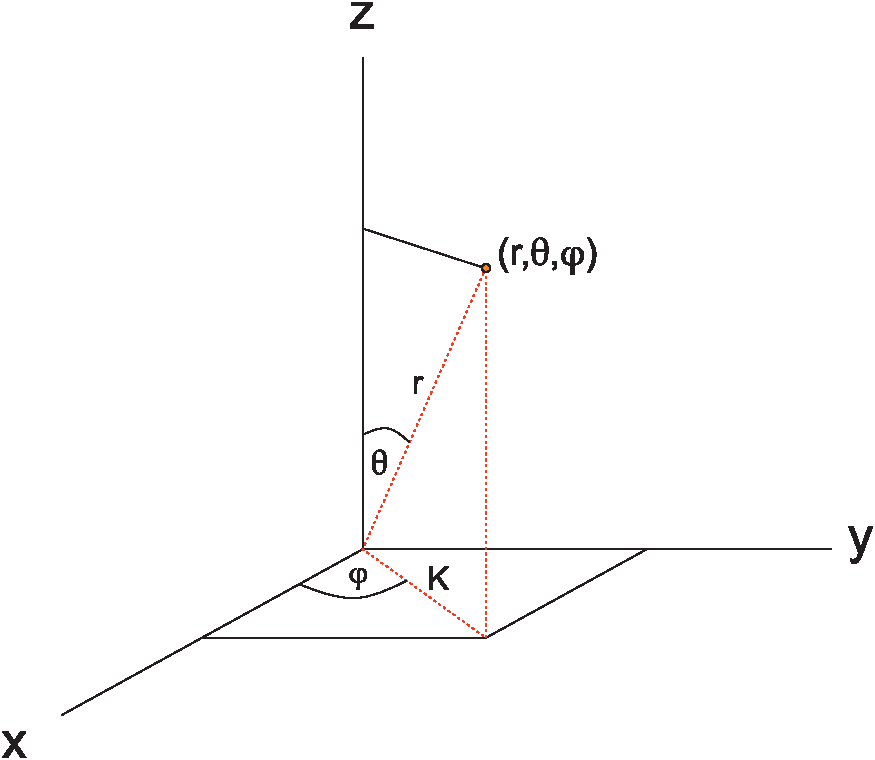
\includegraphics[scale=1.0,angle=0,width=0.8\linewidth]{obrazky-figures/geometry}
	\caption{Výpočet jednotlivých bodů geometrie}
	\label{fig:geom}
\end{figure}
 
Na základě vypočtených úhlů, je možné již spočítat jednotlivé složky kartézské soustavy souřadnic \texttt{[x,y,z]} každému bodu, čímž dojde ke kompletní aproximaci tělesa.

%=========================================================================
\newpage

K výpočtu využijeme goniometrické funkce  a vztahy v pravoúhlém trojúhelníku. Jelikož $ \cos (\varphi) $ je dána poměrem délky přilehlé odvěsny a přeponou \cite{Goniometrie}, tak souřadnici \texttt{\textit{x}} definujeme vtahem:
 
\begin{equation}
 \cos (\varphi) = \frac{x}{K}  \Rightarrow x = \cos (\varphi) \cdot K
\end{equation}
\\
Ze vzniklého vztahu jasně vidíme, že je třeba dopočítat přeponu \textit{K} v trojúhelníku  o stranách $\arrowvert xKy\arrowvert$, kterou ale odvodíme vztahem odvěsny \textit{K} v trojúhelníku $\arrowvert zrK\arrowvert$. Mezi odvěsnou \texttt{K}\footnote{Z obrázku \ref{fig:geom} je patrné, že je přeponou v $\bigtriangleup xKy$, ale odvěsnou v $\bigtriangleup zrK$} a protilehlou přeponou \textit{r} platí, že délka odvěsny protilehlé k úhlu $\varphi$ a délka přepony \cite{Goniometrie} mají vztah:
\\
\begin{equation}
\label{math:K}
\sin (\theta) = \frac{K}{r}  \Rightarrow K = \sin (\theta) \cdot r
\end{equation}
\\
Všechny neznáme máme již dopočítané a můžeme dosadit do první rovnice, čímž dostáváme výsledný vztah převedené souřadnice z kartézské soustavy souřadnic do sférického souřadného systému:
\\
\begin{equation}
\label{math:x}
x = \sin (\theta) \cdot  \cos (\varphi) \cdot r
\end{equation}
\\
Následující souřadnici \texttt{y} vyjádříme obdobným vztahem jako u předchozí souřadnice, ale s tím rozdílem, že protilehlá odvěsna bude k úhlu $\varphi$ a přeponou bude strana \texttt{K}:
\\
\begin{displaymath}
\sin (\varphi) = \frac{y}{K}  \Rightarrow y = \sin (\varphi) \cdot K
\end{displaymath}
\\
Opět máme v rovnici pro výpočet souřadnice \texttt{y} stranu \texttt{K}, kterou ale máme již vypočtenou ve vztahu \ref{math:K}, tudíž už jen tento vztah dosadíme a vznikne výsledná rovnice hledané  souřadnice:
\\
\begin{equation}
\label{math:y}
y = \sin (\varphi) \cdot \sin (\theta) \cdot r
\end{equation}
\\
Poslední souřadnice \texttt{z} je značně jednodušší, protože nám odpadá proměnná \texttt{K}. Vyjádření souřadnice \texttt{z} je principiálně úplně stejné, jako tomu bylo u souřadnice \texttt{x} - přilehlá odvěsna k úhlu $\varphi$ ku přeponě \texttt{r}. Výsledný vztah je tedy možné vyjádřit následovně:
\\
\begin{equation}
\label{math:z}
\cos (\theta) = \frac{z}{r} \Rightarrow z = \cos (\theta) \cdot r
\end{equation}

%=========================================================================
\newpage


\subsection{Vrcholy}
Jakmile máme vypočítány konkrétní složky trojrozměrného prostoru - tedy kompletně spočtený sférický souřadný systém, můžeme přistoupit ke kompletaci dat určených k nahrání do grafické karty. Těmito daty jsou vrcholy samotné geometrie, texturovací data a indexy. 

Získání samotného vrcholu lze vynásobením složek \texttt{x}, \texttt{y} a \texttt{z} průměrem tělesa \texttt{r}. Tato operace musí být provedena u všech bodů koule.

Vzniklé těleso vyobrazené pomocí čar\footnote{Použito grafické primitivum \texttt{gl.LINES}.} je demonstrováno na obr. \ref{img:3}.


\begin{figure}[h]
	\label{img:3}
	\centering
	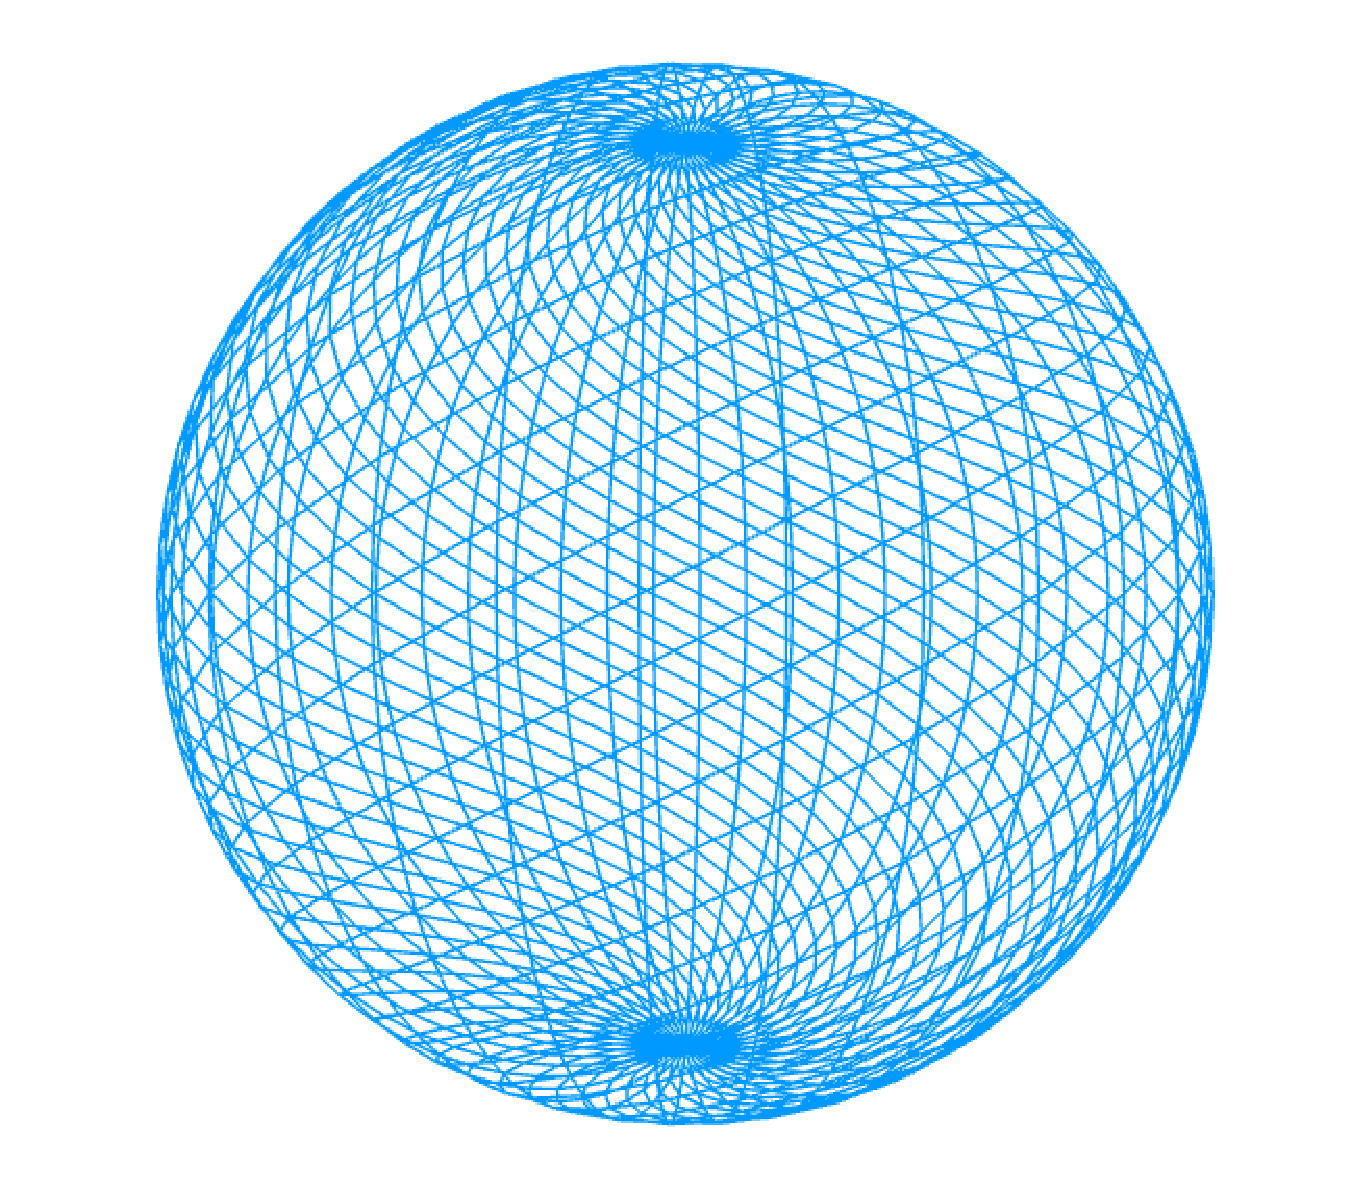
\includegraphics[scale=1.0,angle=0,width=0.7\linewidth]{obrazky-figures/vertex}
	\caption{Koule vyobrazena pomocí čar}
	\label{fig:geom2}
\end{figure}


\subsection{Textura}
Data textury se počítají oproti vrcholům zcela odlišně. Všechny body textur jsou v současné stabilní verzi WebGL pouze dvojrozměrné, tudíž souřadnice \texttt{z} nebudeme potřebovat.
Počet bodů textury bude přímo záviset na počtu rovnoběžek a poledníků.

Od zvoleného počtu rovnoběžek a poledníků se bude dále odvíjet počet bodů textury tak, že pro každou rovnoběžku se spočítají všechny poledníky. Celkový počet bodů textury bude tedy: \textit{počet\_rovnoběžek $\cdot$ počet\_poledníků}.

%=========================================================================
\newpage

Pro lepší představu mapovaní textury můžeme jak poledníky, tak rovnoběžky znázornit ve dvourozměrném prostoru, kde jednotlivé průsečíky tvoří body textury, přičemž horizontální čáry prezentují souřadnici s označením \texttt{\textbf{u}}. Vertikální čáry zase souřadnici \texttt{\textbf{v}}. 

Znázornění demonstruje obrázek \ref{img:grid}. Souřadnici \texttt{\textbf{u}} spočteme vydělením \textit{k}-tého poledníku celkovým počtem poledníků. Souřadnici \texttt{\textbf{v}} vydělením \textit{k}-té rovnoběžky celkovým počtem rovnoběžek.

\begin{figure}[h]
	\label{img:grid}
	\centering
	
\includegraphics[scale=1.0,angle=0,width=0.4\linewidth]{obrazky-figures/grid}
	\caption{Mapování textury}
\end{figure}


\subsection{Indexy}
Zavádění indexů se vyplatí tehdy, pokud chceme vykreslování objektu zefektivnit z hlediska vykreslování jednotlivých bodů. V případě, že se při vykreslování nepoužívá index buffer, tak se pro každé vykreslované primitivum načítá adekvátní počet vrcholů. Potíž nastává v situaci, kdy je vrcholy společný. Dojde k tomu, že souřadnice vrcholu jednoho bodu bude v paměti vícekrát a bude volán pro každé primitivum zvlášť. Díky indexům je pro danou geometrii zmíněn sdílený bod právě jednou, v index bufferu je tento bod zmíněn vícekrát, ale odpovídá mu právě jeden bod geometrie. Díky tomuto odkazování se nám sníží počet vykreslovaných bodů. Indexování se používá spolu s funkcí \texttt{drawElements()} a pro účely implementace bude využita pro zrychlení načítání ekvidistantního zobrazení textur.

%=========================================================================
\newpage

\subsubsection{Návrh index bufferu}
Rovnoběžky a poledníky využijeme i v této části. Jak lze z obrázku \ref{img:grid} pozorovat, horizontální a vertikální čáry tvoří mezi sebou čtvercovou síť, kdy čtverec můžeme snadno interpretovat pomocí trojúhelníku jako grafického vykreslujícího primitiva víz obr. \ref{img:indexes}.



\begin{figure}[h]
	\label{img:indexes}
	\centering
	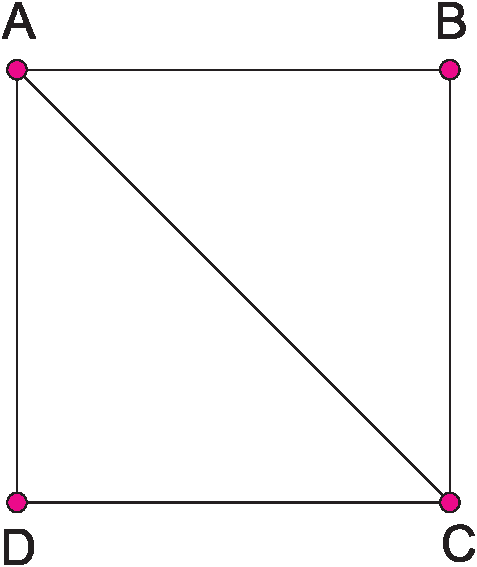
\includegraphics[scale=1.0,angle=0,width=0.5\linewidth]{obrazky-figures/indexes}
	\caption{Implementace indexů}
\end{figure}

Je tedy jasně patrné, že čtverec budeme vykreslovat trojúhelníky $ABC$ a $ADC$. Horizontální přímky protínající body \textit{A}, \textit{B} a \textit{D}, \textit{C}   jsou rovnoběžky, po kterých se budeme při výpočtu bodů posouvat. Naproti tomu body \textit{A},\textit{D} a \textit{B}, \textit{C} prochází poledníky, díky kterým budeme při výpočtu realizovat vertikální posuv.

Samotné zpracování indexů tedy probíhá tak, že pro každou rovnoběžku procházíme její průsečíky s danými poledníky, do index bufferu uložíme pro každé grafické primitivum trojici bodů, což tedy v praxi znamená šestici bodů pro každý čtverec sítě, kde se budou vždy dva body opakovat.

%=========================================================================
\newpage

\section{Korekce textur}
Základní mapování textury lze pozorovat na obr. \ref{img:grid}, takové mapování lze využít u equirectangulárního prohlížení, kde samotná vstupní textura má jíž vše potřebné a není tedy již potřeba nic upravovat - samotná ekvidistantní projekce je převod tělesa trojrozměrného zobrazení do 2D, proto přímo koreluje s daty textury. Pro mód rybího oka je situace složitější, protože vstupní textura není v equirectangulárním modu a naším úkolem je udělat korekci textury tak, aby se textura namapovala na kouli co nejpřesněji.


\begin{figure}[h]
	\label{img:texture_without_correction}
	\centering
	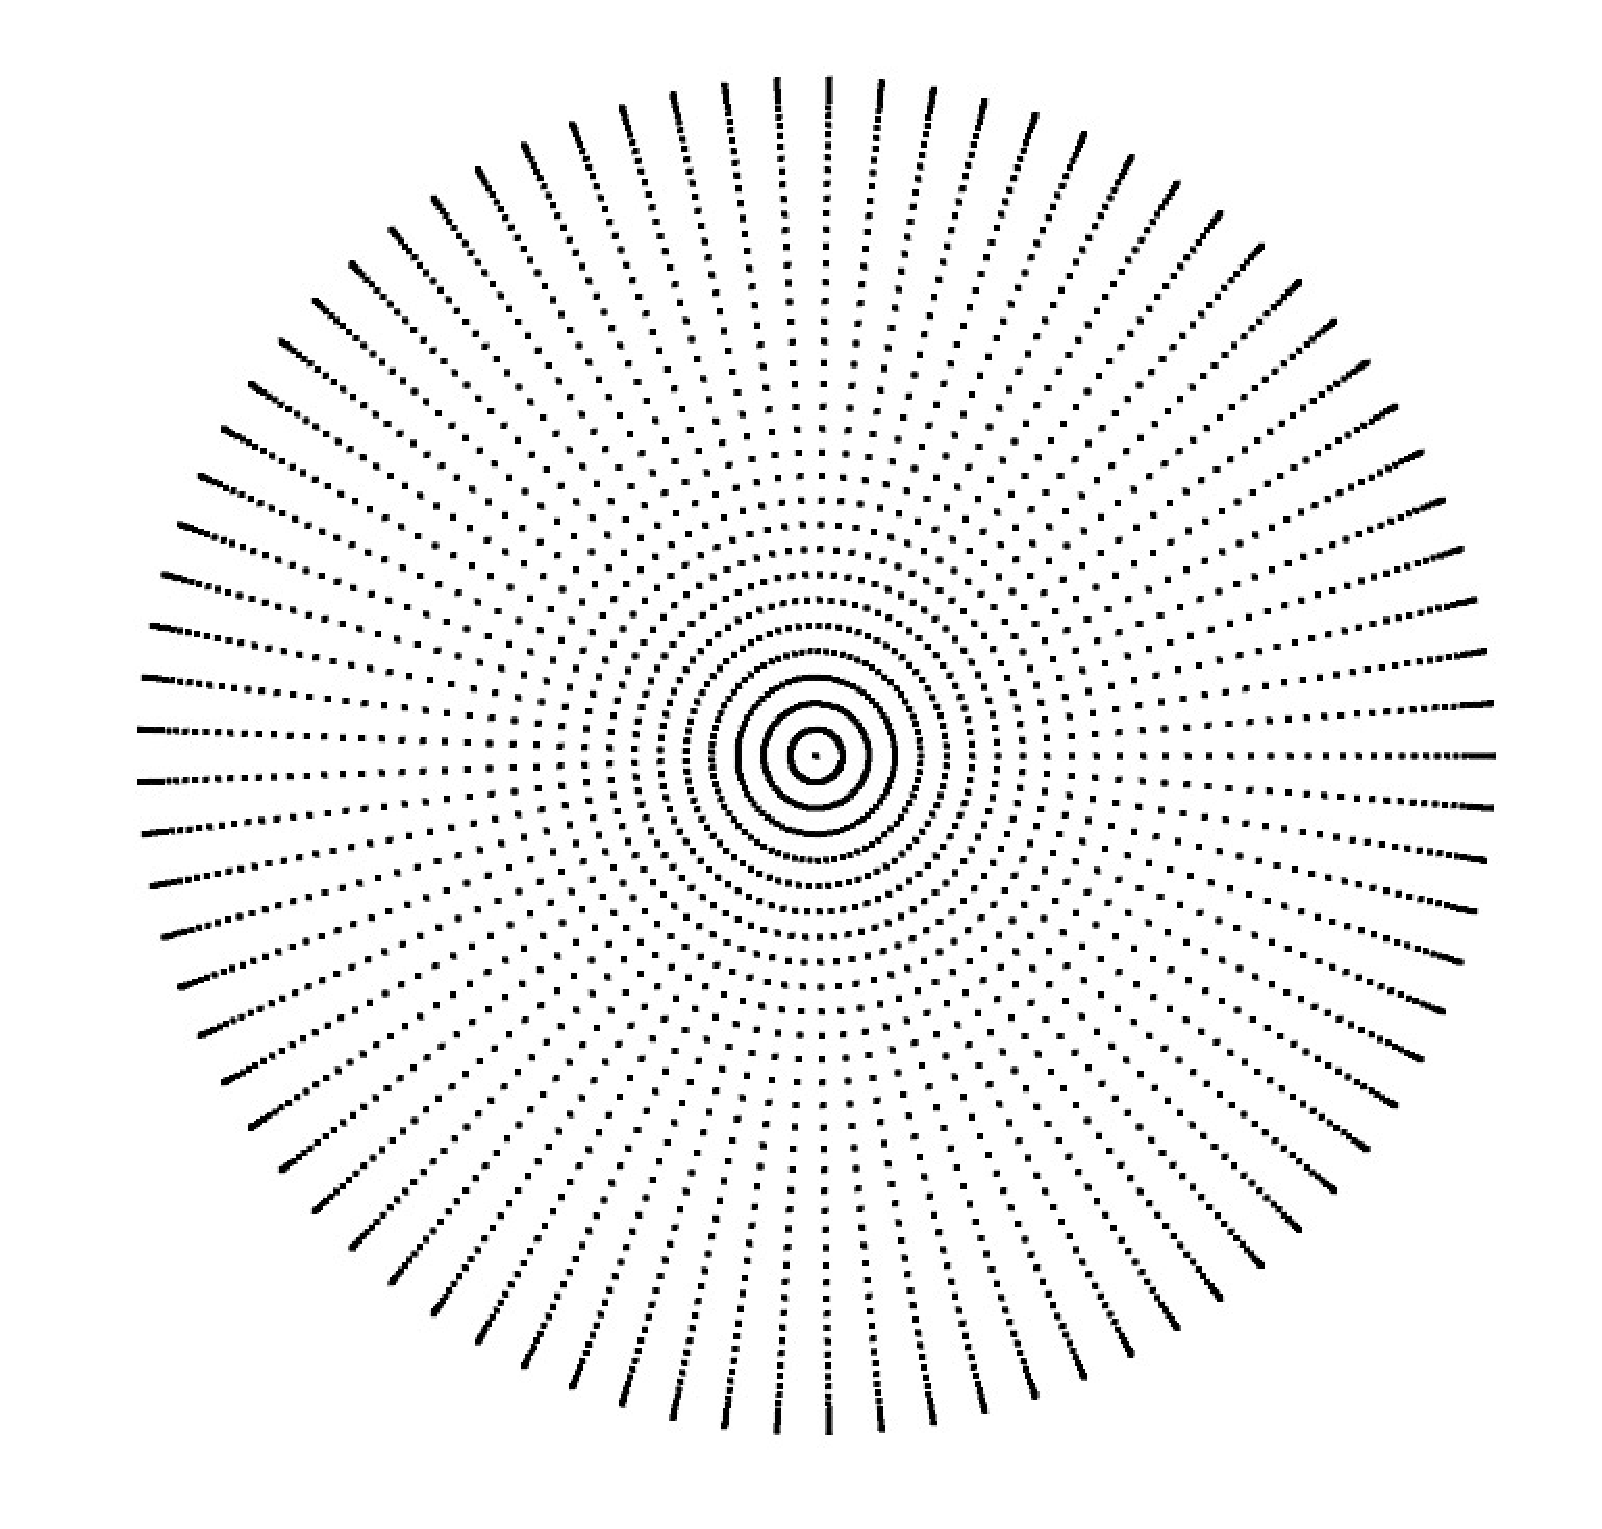
\includegraphics[scale=1.0,angle=0,width=0.6\linewidth]{obrazky-figures/texture}
	\caption{Textura vycházející z předpočítaných dat. Bez korekce.}
\end{figure}

\section{Korekce pro rybí oko}
Korekci využijeme především k tomu, aby se nám textura mapovala přesněji v oblasti švu, tedy přesně v polovině tělesa. Důvodem je ten, že pokud bychom korekci textury neudělali, okraje by byly rozostřené  a v oblasti švu data hůře čitelná.  Samotná korekce nemá na funkci prohlížení žádný vliv.
S korekcí se mapuje textura daleko přesněji, resp. okraje hemisféry. Na obrázku \ref{img:texture_without_correction} si lze povšimnout ukázky dat textury ještě před provedením korekce krajních bodů.

Pro výpočet korekce můžeme využít jako počáteční hodnoty souřadnic již ty spočítané pro normály\footnote{V našem případě hodnota souřadnice vrcholu podělená průměrem tělesa.} popř. vrcholy geometrie.

Již před-počítané hodnoty je ale nutné ještě upravit, protože jsou počítány pro trojrozměrný prostor a my pro texturu potřebujeme pouze dva rozměry. Úpravou je v tomto smyslu myšleno to, že velikost poloměru  kružnice se bude měnit rovnoměrně, tedy hlavně u bodů, které odpovídají bodům v oblasti švu, v tomto místě dochází k největšímu zhuštění bodů, což má za následek již avizované neúměrné roztažení a deformaci textury.
%=========================================================================
\newpage




Je-li  souřadnice \textit{\textbf{\axisY}} definována rovnicí \ref{math:\axisY} a souřadnice \textit{\textbf{\axisZ}} vztahem \ref{math:\axisZ}, tak korekce textury bude realizována vynásobením  vertikální a horizontální souřadnice funkcí \textit{\textbf{arccos(\axisY)}}. Každá hemisféra koule bude mít odlišnou modifikaci souřadnice \texttt{\textbf{\axisX{}}}, resp. výpočet každé hemisféry probíhá v jiném kvadrantu kartézské soustavy souřadnic. V opačném případě bychom nemohli mapovat obě sféry, protože by se nám spojily do jedné tj. body by se překrývaly - důvod je zřejmý, data z kterých korekce vychází jsou počítány pro celou kouli a nerespektováním změny souřadnice, by se bod zobrazil až  ``za'' vyobrazeným bodem na obrazovce\footnote{Z pohledu na těleso ve 3D.}. \\

Horizontální a vertikální souřadnici \texttt{\textbf{u}} a \texttt{\textbf{v}} spočítáme následujícím způsobem:




\begin{itemize}
	\item Pro levou hemisféru bude platit následující vztah:\\
		    $$u =  \axisX{} \cdot \frac{\arccos(\axisY{})}{r} \wedge v =  \axisZ{} \cdot \frac{\arccos(\axisY{})}{r}$$   
		   
	\item Pravá hemisféra je difinována vztahem:\\
			$$u =  -\axisX{} \cdot \frac{\arccos(\axisY{})}{r}\wedge v =  \axisZ{} \cdot \frac{\arccos(\axisY{})}{r} $$ 
 
\end{itemize}
 

\begin{figure}[h]
	\label{img:texture_with_correction}
	\centering
	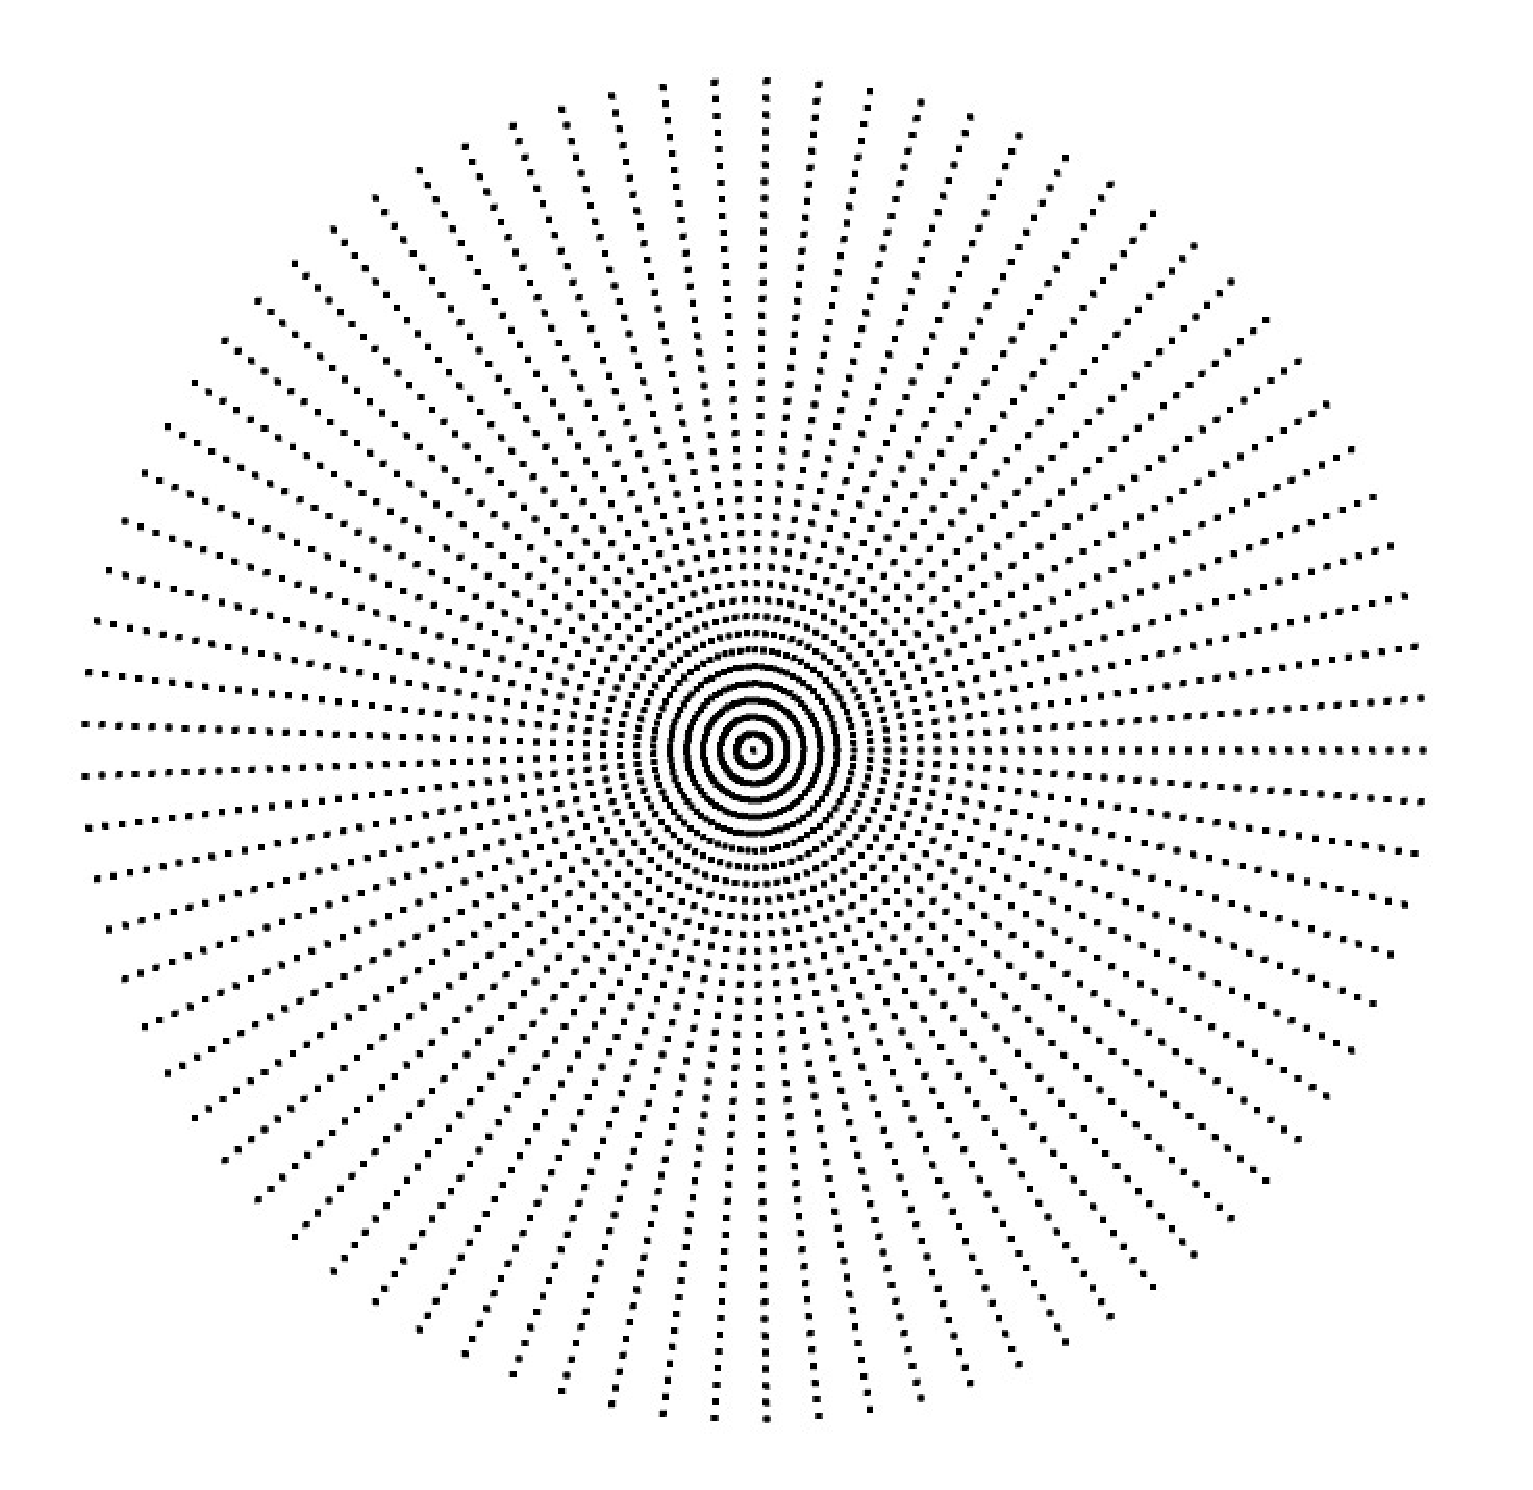
\includegraphics[scale=1.0,angle=0,width=0.6\linewidth]{obrazky-figures/texture_correction}
	\caption{Textura s korekcí krajních bodů.}
\end{figure}

Proměnná \texttt{r} označuje poloměr koule, resp. kružnice ve 2D. Obrázek \ref{img:texture_with_correction} demonstruje již aplikovanou  korekci vstupních dat  textury z obr. \ref{img:texture_without_correction} avizovanou výše.
 

%=========================================================================
\newpage


\section{Návrh projekce}
Součástí již avizované projekce v předchozí kapitole, jsou matice, které modelovou, zobrazovací a projekční matici utváří. Mezi ně patří např. rotační matice po osách \texttt{x},\texttt{y} a \texttt{z}, matice posuvu, změny měřítka apod. Díky těmto maticím jsem schopni projekci zrealizovat - kdy v perspektivním pojetí vyváříme frustrum\footnote{V ortografickém zobrazení by to byl kvádr/krychle.}, resp. komolý jehlan, kdy stěny tvoří lichoběžník a obě podstavy čtverec popř. obdélník. Veškeré vykreslovaná data, která neleží v komolém jehlanu jsou ořezány  a nebudou vykreslena. 





\subsection{Modelová matice}
Sem patři rotační matice všech os souřadného systému, dále matice pro změnu měřítka souřadnic a posuvná matice objektu.

Cílem modelové matice je tedy transformovat body modelu ze středu souřadného systému, vůči kterému byly body geometrie modelu napočítány, do zobrazitelného prostoru, se kterým budeme dále pracovat. Cílem modelové matice je posunout a pootočit zobrazovaným objektem do výchozí pozice promítání. Otáčení apod. operace v reálném čase jsou  doménou zobrazovací matice. Začneme s matici pro změnu měřítka modelu:

$$
S =
\begin{pmatrix} 
\textbf{x} & 0 & 0 & 0\\
0 & \textbf{y} & 0 & 0\\ 
0 & 0 & \textbf{z} & 0\\ 
0 & 0 & 0 & 1\\ 
\end{pmatrix}$$


Matice rotace kolem osy x:

$$
R_{x}=
\begin{pmatrix} 
	1 & 0 & 0 & 0\\
	0 & \cos(\alpha) & -\sin(\alpha) & 0\\ 
	0 & \sin(\alpha) & \cos(\alpha) & 0\\ 
	0 & 0 & 0 & 1\\ 
\end{pmatrix}$$

Matice rotace kolem osy y:

$$
R_{y}=
\begin{pmatrix} 
 \cos(\alpha) & 0 & \sin(\alpha) & 0\\
0 & 1 & 0 & 0\\ 
-\sin(\alpha) & 0 & \cos(\alpha) & 0\\ 
0 & 0 & 0 & 1\\ 
\end{pmatrix}$$

Matice rotace kolem osy z:

$$
R_{z}=
\begin{pmatrix} 
\cos(\alpha) & -\sin(\alpha) & 0 & 0\\
\sin(\alpha) & \cos(\alpha) & 0 & 0\\ 
0 & 0 & 1 & 0\\ 
0 & 0 & 0 & 1\\ 
\end{pmatrix}$$

Matice pro posun objektu po osách \texttt{x},\texttt{y} a \texttt{z}. Přímo vychází z identické matice\footnote{Na hlavní diagonále jsou jedničky, všude jinde nuly.}:

$$
T =
\begin{pmatrix} 
1 & 0 & 0 & 0\\
0 & 1 & 0 & 0\\ 
0 & 0 & 1 & 0\\ 
\textbf{x} & \textbf{y} & \textbf{z} & 1\\ 
\end{pmatrix}$$

%=========================================================================
\newpage

Výsledná modelová matice \texttt{\textbf{M}} je tedy dána vztahem:
$$ M = T \cdot R_{x} \cdot R_{y} \cdot R_{z} \cdot S $$

Při násobení původní matice rotační maticemi hrají  velkou roli také znaménka. Jelikož v implementační části budeme používat interakce s myší a tím měnit náhled pozorovatele resp. kamery na náš model, bude třeba zvolit směr posuvu zorného pole kamery. 

Vlastnosti prohození znamének využijeme právě u  rotace $R_{x}$ a $R_{y}$, které reprezentují pohyb myši.  


\subsection{Zobrazovací matice}
Jedná se o matici, která kontroluje způsob, jakým se na objekt díváme. V našem konkrétním případě budeme view matrix používat k napodobeni pohybu kamery snímající objekt, jak je tomu v reálném světě. 

Prostor objektu, který jsme pomocí modelové matice transformovali do zobrazitelného prostoru musíme nyní převést do prostoru, který bude relativní vzhledem k pohledu pozorovatele.

Takového efektu docílíme tak, že složku o kterou se chceme posunout, vynásobíme opačnou hodnotou modelu ve scéně. Výsledný vztah pro výpočet zobrazovací matice tedy je:

$$ V = T \cdot R_{x} \cdot R_{y} \cdot R_{z} $$ 

\subsection{Perspektivní matice}

Jednotlivé argumenty potřebné pro definování perspektivní matice zobrazení:

\begin{description}
		\item[fov] - pole, které definuje zorný úhel
		\item[aspect] - poměr šířky a výšky scény
		\item[near] - reprezentuje rovinu, která ořeže tu část modelu, která je příliš blízko pozorovateli
		\item[far] - reprezentuje rovinu, která ořeže tu část modelu, která je příliš daleko pozorovateli
\end{description}

 
$$
P =
\begin{pmatrix} 
\dfrac{1}{aspect \cdot \tan\left(\dfrac{ fov }{2}\right)} & 0 & 0 & 0\\
0 & \dfrac{1}{\tan\left(\dfrac{ fov }{2}\right)} & 0 & 0\\ 
0 & 0 & \left(\dfrac{near+far}{near-far}\right) & -1\\ 
0 & 0 &  \left(\dfrac{near \cdot far \cdot 2}{near-far}\right)  & 1\\ 
\end{pmatrix}
$$


%=========================================================================
\newpage

\section{Zorný úhel}
Zorný úhel je grafický prvek, který udává informace o aktuálním zorném poli zobrazovací matice. Tento úhel se mění na základě přibližování, nebi oddalování scény od pozorovatele. 

\subsection{Návrh prvku}
K vyobrazení prvku budeme potřebovat vektor svg zobrazující přímý úhel. Reprezentován bude tvarem polokoule, u které se využije vlastnosti tahu. Ve vektorové grafice se jedná o nastavení atributu \texttt{stroke-width}, který bude reprezentovat zorný úhel. Důvodem, přoč pro vyobrazení samotné není využita samotná křivka vyplněná barvou je ten, že pokud se přenastaví úhel zobrazení, tak se křivka zdeformuje tak, že z ní není zjevný zorný úhel.

Vstupními argumenty je pozice prvku pomoci ve dvojrozměrném prostoru \texttt{(x,y)} a průměr kruhu. Dále je potřeba přepočítat tyto souřadnice dvojrozměrného prostoru na sférické souřadnice. K samotnému výpočtu dostačuje Pythagorova věta, kdy pomocí bodu \texttt{(x,y)} jsou známy hodnoty odvěsen a je možní spočítat přeponu. Takto odvodíme vztahy \\pro \texttt{x} a \texttt{y}.


 $$ x = r\cdot\cos(\theta) $$ 
 $$ y = r\cdot\sin(\theta) $$  

 


%=========================================================================
\newpage


\section{Kompas}
Dalším rozšířením prohlížení jsou údaje o světových stranách díky kompasu. Střelka kompasu se bude pohybovat k severu díky vstupním argumentům, které budou předány přímo do programu. Ukazatel severu se bude měnit na základě rozdílu vůči vstupní pozici, která definuje pozici severu ve scéně. Samotna realizace střelky bude díky obrázku \texttt{svg} a natáčení pomocí změně kaskádových stylů. Změna zobrazení bude udávána ve stupních vůči původní pozici. Samotná transformace zobrazení, resp. otočení střelky budeme realizovat pomocí vlastnosti kaskádových stylů \texttt{transform: rotate(\textbf{\emph{X}}deg)} kde \texttt{\textbf{\emph{X}}} je posuv ve stupních.

\subsection{Výpočet posuvu}
Korekce kompasu bude daná úhlem, který svírá střed zorného pole a vstupní statickou pozici zadanou argumentem programu, která po celou dobu běhu programu nad danými daty zůstane neměnná. Tedy samotná korekce bude reagovat pouze na změnu horizontální osy.

\section{Metadata}
\section{Blending}
%=========================================================================

\chapter{Implementace panoramatického prohlížeče}
\label{chapter:4}
V této kapitole rozeberu implementaci programu  spolu s  problémy, které bylo nutné v průběhu implementace řešit. Program se skládá z jazyka HTML5, ve kterém je nastíněna výchozí kostra, nad kterou pracuje veškerá funkcionalita. Jádro je napsáno v jazyce Javascript bez použití frameworků  a  shadery, které jsou implementovány v jazyce GLSL. 


\section{Stavy a data programu}
Jelikož samotná implementace ve WebGL vyžaduje k realizaci problematiky více jazyků, vzniká v programu velké množství proměnných, které je velice vhodné určitým způsobem pro vyšší přehlednost v kódu sdružovat. Program jako takový je napsán procedurálním stylem, ale sám využívá některé objektové vlastnosti. Mezi ně patří právě sdružování proměnných, které jsou hierarchicky uspořádány do objektu.

Každá důležitá část implementace má svůj vlastní objekt proměnných, které se k dané problematice vztahují, včetně všech nutných interních stavů.

\subsection{Myš a klávesnice}
Veškeré interakce s myší se z hlediska datové částí promítají do objektové proměnné \texttt{MOUSE}, která udržuje data o pohybu pozorovatele ve scéně po vertikální a horizontální ose otáčení, včetně hloubky posuvu - tedy přibližování scény pomocí kolečka. Většina udržovaných dat v proměnné \texttt{MOUSE} pochází z objektu \texttt{MouseEvent} popř. \texttt{WheelEvent}. Objekty poté díky Javascriptové metodě \texttt{addEventListener()} uchovávají aktuální hodnoty vstupu odkud se čtou.
Dalším objektem je klávesnice realizována pomocí objektové proměnné \texttt{KEYBOARD}, která udržuje pouze základní informace, zdali je aktivní popř. jaká citlivost pohybu pozorovatele ve scéně pomocí klávesnice má být. Veškeré interakce s klávesnici jsou dále realizovány pomocí čtení z objektu \texttt{KeyboardEvent}, do které se načítají údaje o stisku kláves, tudíž na rozdíl od myši není třeba tyto data uchovávat, protože klávesnice je závislá pouze na aktuálním stavu. 

%=========================================================================
\newpage

\subsection{Data programu a nastavení}
Obdobným způsobem, jak je již nastíněno výše, jsou uchovávány proměnné a nastavení samotného programu. Programová objektová proměnná \texttt{PROG} uchovává data jako jsou buffery programu, transformační matice, nad kterými probíhá projekce a v neposlední řadě atributy shaderů, díky kterým jsou data matic, bufferů apod. nahrávány na grafickou kartu. 

Odděleně od programu je vytvořen objekt geometrie, který počítá a vytváří všechna data spojených s geometrií a mapováním textury pro nahrání na GPU. Objekt vytváří funkce \texttt{\createSphereGeometry}.

Objektová proměnná \texttt{SETTINGS} uchovává informace o nastavení módu programu resp. formát dat, které bude program vyobrazovat. Dále informace pro nastavení a inicializaci grafických prvků.


\section{Běh programu}
Ihned po načtení HTML kostry programu je zavolána hlavní funkce programu \texttt{\main}, která je spuštěna  na základě vyvolání události \texttt{onload()} \footnote{ Událost \texttt{onload()} nastane ihned po načtení webové stránky.} .

Před samotným spuštěním programu je nutné provést některé inicializační operace - nastavení potřebných proměnných pro běh, ověření a ošetření. 

Tuto roli obstarává funkce \texttt{\initProgram}. Je zde nutné ověřit, zdali se podařilo získat WebGL kontext z plátna \texttt{<canvas>}. Pokud by došlo k situaci, že prohlížeč nebude podporovat kontext WebGL, program se ukončí. Mezi další funkce inicializace patří, že na základě vstupu nastaví, jaký mód prohlížení bude zvolen, resp. na základě vstupních proměnných objektu \texttt{SETTINGS}  se nakonfiguruje funkce \texttt{\createSphereGeometry}. 

V případě, že inicializování proběhlo v pořádku, zavolá se funkce \texttt{\setupProgram}, kde dochází k sestavení všech částí programu a nahrání nejdůležitějších dat na grafickou kartu. Dochází zde také ke kompilaci obou shaderů a provázání s programem. Mezi další operace, patří naslouchání vstupních informací z myši, kolečka klávesnice aj.  pomocí metody \texttt{addEventListener()}.

Pokud  \texttt{\setupProgram} proběhne v pořádku a  data jsou připravena, je možné nahrát také texturu - pro panoramata jsou textury nahrávány také z funkce \texttt{\setupProgram}, v případě videa je tato operace  volána z funkce \texttt{\render}, důvodem je ten, že video potřebuje reflektovat změny v čase.



\subsection{Shadery}
\subsection{Transformační matice}
\subsection{Buffery a geometrie}
\subsection{Načítání a vykreslování textur}

\section{Mody prohlížení}

\section{Ovládání myší}

\section{Ovládání klávesnicí}

\section{Grafické rozhraní}
Veškeré prvky, které nejsou vykreslovány skrze grafickou kartu, se v elementu jak již bylo nastíněno v předcházejících kapitolách, \texttt{<canvas>} nezobrazí z důvodu, že je vše skryto. Jen v případě, že by prohlížeč nepodporoval plátno, zobrazí co je v něm. Realizaci samotných prvků jako je kompas, nebo zorný úhel až po ovládací prvky videa, bude třeba realizovat za pomocí kaskádových stylů, kdy pomocí dynamického pozicování budeme všechny prvky zobrazovat překryvem plátna.

\section{Kompas}
Prvek překrývající plátno \texttt{<canvas>}. Vstupnímí metadaty jsou zadány koordinační body severu, popř. jihu. Díky interakcí s myší - tedy násobení zobrazovací transformační maticí realizujeme pohyb pozorovatele, čímž se mění prostorové úhel, který ovlivňuje odchylku severu, popř. jihu od původní zadané pozice v metadatech.

Samotná konstrukce kompasu je zasazena do tagu \texttt{<div id="compass-box">}. Funkce, která nahraje data do kontejneru kompasu se nazývá \texttt{createCompass()}.

\subsection{Pozicování}
Vytvoření samotného kompasu realizuje funkce \texttt{createCompass(width, height)}, argument \texttt{width} udává šířku kompasu, argument \texttt{height} zase jeho výšku. Pozice kompasu v plátně je realizována pomocí nastavení hodnot \texttt{div.style.left} a 
\texttt{div.style.top} v pixelech, kde se bude udávat výsledná hodnota posuvu. Pozici samotnou nastavuje řádek \texttt{div.style.position = 'absolute';}. Posun  od levého okraje obrazovky \texttt{div.style.left} je vypočten tak, že si načteme celkovou šířku

\section{Zorný úhel}



Pravidla \cite{Kompendium}. Pravidla \cite{Goniometrie}. 
Goniometrie


%=========================================================================
\newpage

\chapter{Testování}
\label{chapter:5}
\section{Windows a linux}
\section{Prohlížeče a kompatibilita}


\chapter{Závěr}
\label{chapter:6}

Závěrečná kapitola obsahuje zhodnocení dosažených výsledků se zvlášť vyznačeným vlastním přínosem studenta. Povinně se zde objeví i zhodnocení z pohledu dalšího vývoje projektu, student uvede náměty vycházející ze zkušeností s řešeným projektem a uvede rovněž návaznosti na právě dokončené projekty.

%=========================================================================
